% What's SQL
% Tools to use SQL
% Alternatives
% Why we will focus on SGDB
\begin{frame}
  \frametitle{Qu'est-ce que SQL?}

  SQL (Structured Query Language) est un langage de programmation utilisé pour gérer et manipuler des bases de données relationnelles.

  \begin{itemize}
      \item Permet d'interroger des bases de données
      \item Utilisé pour créer et modifier des schémas de bases de données
      \item Standard de l'industrie pour les bases de données relationnelles
  \end{itemize}
\end{frame}

\begin{frame}
  \frametitle{Vocabulaire SQL et Bases de Données}

  \begin{description}
    \item[Base de Données (Database)] Une collection organisée d'informations structurées ou de données.
    \item[Table] Une structure qui contient des données sous forme de lignes et de colonnes.
    \item[Colonne (Field)] Un élément de données d'un certain type dans une table.
    \item[Ligne (Record)] Une entrée individuelle dans une table.
    \item[Clé Primaire (Primary Key)] Une colonne (ou un ensemble de colonnes) dont chaque valeur est unique et identifie une seule ligne de la table.
    \item[Clé Étrangère (Foreign Key)] Une colonne (ou un ensemble de colonnes) qui référence la clé primaire d'une autre table.
  \end{description}

\end{frame}

\begin{frame}
  \frametitle{Vocabulaire SQL et Bases de Données}

  \begin{description}
    \item[Requête (Query)] Une instruction pour la base de données pour récupérer ou manipuler des données.
    \item[Jointure (Join)] Une opération qui combine des données de deux tables en fonction d'une relation entre elles.
    \item[Indice (Index)] Une structure qui améliore la vitesse des opérations sur une table.
    \item[Contrainte (Constraint)] Une règle appliquée aux données lors de leur insertion, mise à jour ou suppression.
  \end{description}

\end{frame}


\begin{frame}
  \frametitle{Outils SQL}

  Les outils SQL offrent une interface pour travailler efficacement avec des bases de données SQL.

  \begin{itemize}
      \item \textbf{SGBD (Systèmes de Gestion de Bases de Données)} : Comme MySQL, PostgreSQL, Oracle, et SQL Server.
      \item \textbf{Outils GUI}: Des interfaces graphiques telles que SQL Server Management Studio, DBeaver, et phpMyAdmin pour faciliter la gestion.
      \item \textbf{ORM (Object-Relational Mapping)}: Frameworks comme Hibernate ou SQLAlchemy qui mappent les objets de code aux données de la base.
      \item \textbf{Outils d'analyse et de reporting}: Tels que Tableau ou Microsoft Power BI qui peuvent se connecter directement à des bases SQL pour l'analyse.
      \item \textbf{Outils de migration et de versioning}: Comme Flyway ou Liquibase pour gérer les évolutions du schéma de base de données.
  \end{itemize}
\end{frame}

\begin{frame}
  \frametitle{Alternatives à SQL}

  \begin{itemize}
      \item \textbf{Document} : Bases de données comme MongoDB qui stockent des données sous forme de documents, généralement en JSON.
      \item \textbf{Colonne}: Solutions comme Cassandra ou HBase, conçues pour stocker et traiter de grands volumes de données sur de nombreux serveurs.
      \item \textbf{Clé-Valeur}: Bases de données comme Redis ou DynamoDB, optimisées pour les opérations de récupération rapide par clé.
      \item \textbf{Graphes}: Neo4j ou OrientDB qui sont optimisés pour stocker des données interconnectées et réaliser des requêtes complexes sur ces relations.
      \item \textbf{Recherche textuelle}: ElasticSearch ou Solr, qui sont optimisés pour la recherche textuelle et l'analyse de données.
      \item \textbf{Vecteurielles}: FaunaDB ou Milvus, conçues pour des recherches basées sur la similarité de vecteurs, idéales pour la recherche d'images, audio, ou texte à grande échelle.
  \end{itemize}
\end{frame}

\begin{frame}
  \frametitle{Pourquoi connaître SQL malgré les alternatives?}

  \begin{itemize}
      \item \textbf{Ubiquité}: SQL est la norme de facto pour les bases de données relationnelles depuis des décennies. La majorité des entreprises ont des bases de données SQL en production.
      \item \textbf{Transversalité}: La connaissance de SQL est souvent requise pour des rôles variés : développeurs, analystes de données, administrateurs de bases de données, et plus encore.
      \item \textbf{Intégration}: Beaucoup d'outils et de technologies modernes, même ceux axés sur NoSQL, offrent une interface SQL ou une compatibilité SQL.
      \item \textbf{Maturité}: SQL a été testé et optimisé pendant des années, avec une vaste documentation, des communautés d'utilisateurs, et de nombreux outils de support.
      \item \textbf{Raisonnement structuré}: Apprendre SQL renforce une manière structurée de penser à la manipulation des données, ce qui est bénéfique même lors de l'utilisation d'autres technologies.
  \end{itemize}
\end{frame}

\begin{frame}
  \frametitle{Différents SGBD}

  \begin{columns}[T,onlytextwidth]
    \column{0.25\textwidth}
      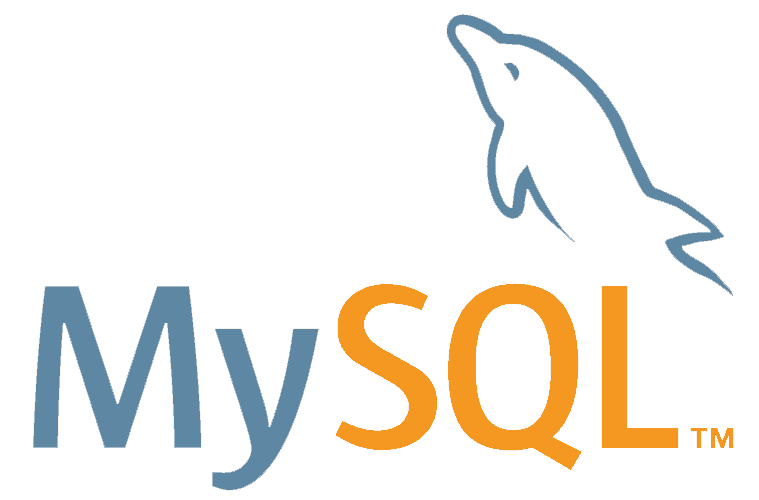
\includegraphics[width=0.8\linewidth]{mysql-logo.png} \\
      MySQL

    \column{0.25\textwidth}
      
\includegraphics[width=0.8\linewidth]{pg.png} \\
      PostgreSQL

    \column{0.25\textwidth}
      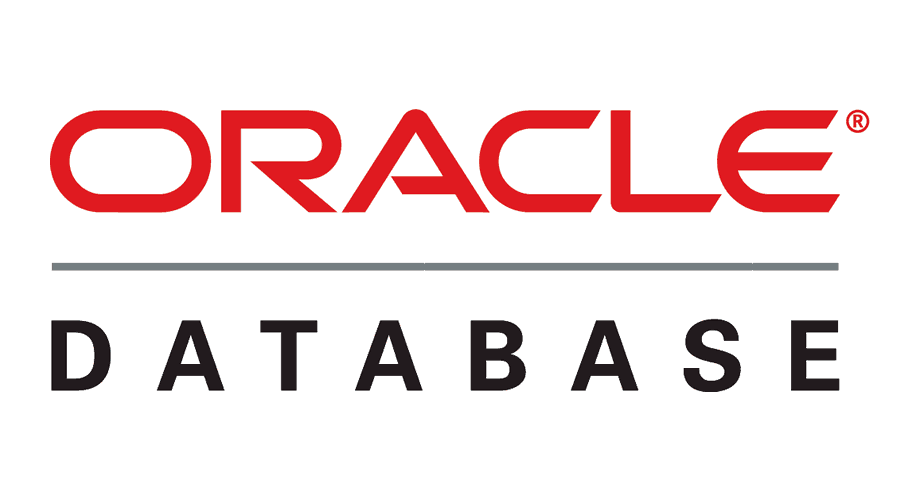
\includegraphics[width=0.8\linewidth]{oracle-database-logo.png} \\
      Oracle

    \column{0.25\textwidth}
      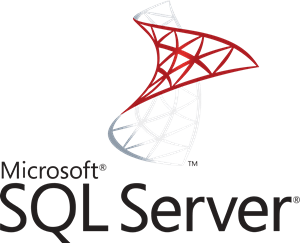
\includegraphics[width=0.8\linewidth]{microsoft-sql-server-logo-96AF49E2B3-seeklogo.com.png} \\
      SQL Server
  \end{columns}

  Chaque SGBD a ses propres avantages, fonctionnalités, et utilisations spécifiques.

\end{frame}
